\section{Sistemas de Control de Versiones Distribuidos DCVS}
\subsection{Introducción}
Los DVCS son herramientas de control de versiones que toman un enfoque punto a punto (peer to peer), al contrario de los centralizados que toman 
un enfoque cliente-servidor. Con ellos solo se mantiene una copia local del repositorio, pero cada equipo se convierte en un \textbf{repositorio} del
resto de usuarios, esto permite una fácil bifurcación en ramas y un manejo más flexible del repositorio.
En este sistema existen pocos comandos que no trabajen directamente con el propiop disco duro, lo que lo covierte en una herramienta más rápida
que un \textbf{Sistema de Control de Versiones Centralizado}. Cuando hayamos decidido que estamos listos, podemos enviarles los cambios a los repositorios de 
los otros usuarios. Otra de las ventajas de trabajar de forma local es que puedes trabajar sin conexión a la red.
En este sistema es importante la diferencia entre ramas de desarrollo (destinadas a pruebas, inestables, etc...) y la rama principal (trunk/master),
en principio la actualización del repositorio se llevará a cabo de la rama principal y no del resto de ramas, aunque últimas si que pueden
actualizarse en repositorios externos.

\subsection{Diferencias entre DCVS y CVS}
Las principales diferencias entre un sistema centralizado y uno distribuido son las siguientes, algunas ya señaladas en la introducción:
\begin{enumerate}
\item No existe una copia de referencia del código, solo copias de trabajo.
\item Las operaciones suelen ser más rápidas al no tener que comunicarse con un servidor central.
\item Cada copia de trabajo es un tipo de respaldo del código base.
\item No hay que hacer update antes del commit, se trabaja sobre copia local.
\item Se eliminan los problemas de latencia de la red.
\item La creación y fusión de ramas es más fácil, porque cada desarrollador tiene su propia rama.
\end{enumerate}

Las principales desventajas que encontramos son las siguientes:
\begin{enumerate}
\item Todavía se necesita un sistema de backup. No hay que fiarse de que el backup reside en otro usuario, ya que este puede no admitirte más,
o estar inactivo mientras que yo tengo cambios hechos, por lo que todavía será necesario un servidor central donde realizar los backups.
\item Realmente no hay una \textit{última versión}. Si no hay un repositorio central no hay manera de saber cuál es la última versión estable del producto.
\item Realmente no hay números de versión. Cada repositorio tiene sus propios números de revisión dependiendo de los cambios. En lugar de eso, 
la gente pide la última versión del guid (número de versión) concreto, aunque cabe la posibilidad de etiquetar cada versión.
\end{enumerate}

Encontramos dos nuevos comandos principales que no trabajan localamente:
\begin{itemize}
\item push: envía cambios a otro repositorio (por supuesto, requiere permisos).
\item pull: obtiene los cambios de otro/s repositorios.
\end{itemize}


\subsection{Cómo funcionan}
Como se ha dicho cada desarrollador tiene su repositorio local si un usuario A realiza un cambio lo hace localemente y cuando crea oportuno puede
compartirlo con el resto de usuarios. Pero existe una duda: ¿cuál es la versión principal?, la respuesta es sencilla: existe una rama principal
en la cual todos los usuarios registran los cambios realizados obteniendo de esta forma la versión final. 
Para más detalles explicaremos esto de forma gráfica como se muestra en la  Figura~\ref{fig:01}.

%\begin{figure}
%  \centering
%    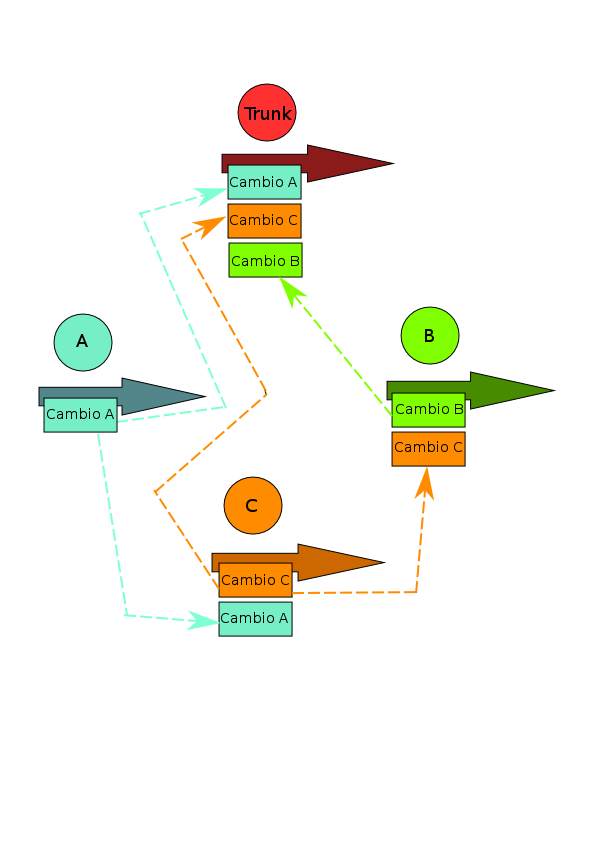
\includegraphics[width=0.5\textwidth]{./imagenes/graficodist.png}
%  \caption{DCVS}
%  \label{fig:01}
%\end{figure}

En el gráfico podemos ver la rama principal (trunk) y varios usuarios (A, B, y C). Cada usuario tiene su propio repositorio con ciertas ramas de
desarrollo, existe una rama principal que lleva las versiones oficiales y sin fallos. Cada usuario guarda su copia local, pero además envía y 
recibe desde y a otros repositorios ciertas ramas de desarrollo y por supuesto la principal que es la que contiene las versiones estables del 
proyecto.

\subsection{Diferentes DCVS}
Entre los más populares encontramos:
\begin{itemize}
\item Git
\item Mercurial
\item Baazar
\item Darcs
\item Monotone
\end{itemize}
Procedemos a explicar Git y Mercurial al ser los más utilizados actualmente. 


\subsection{GIT}
Git es uno de los sistemas de control de versiones distribuidos más usados. Git fue creado por Linus Torvalds y buscaba un sistema que cumpliera
4 requisitos básicos:
\begin{itemize}
\item No se pareciera a CVS
\item Fuera distribuido
\item Seguro frente corrupción, accidental o intencionada
\item Gran rendimiento en las operaciones
\end{itemize} 
Git está escrito en C y en gran parte fue construido para trabajar en el kernel de Linux, lo que quiere decir que desde el primer día ha tenido que mover 
de manera efectiva repositorios de gran tamaño. 

\subsubsection{GIT Es Distribuido}
Cada usuario tiene una copia completa del servidor principal, y cualquiera de ellas podría ser recuperada para reemplazarlo en caso 
de caída o corrupción. Básicamente, no hay un punto de fallo único con git a no ser que haya un punto único. 
\subsubsection{Ramas Locales Sin Coste}
Posiblemente la razón más fuerte a favor de Git que realmente lo hace destacar de casi cualquier otro SCV es su modelo de ramas. Git permite
tener múltiples ramas locales independientes entre sí y se tarda segundos en crear, fusionar, o borrar estas líneas de desarrollo.
Se pueden hacer cosas como: 
\begin{itemize}
\item Crear una rama para probar una idea, volver al punto desde el cual bifurcaste y volver a donde estabas experimentado y fusionarlo. 
\item Tener una rama que siempre contiene sólo lo que va a producción, otra en la que acumulas el trabajo para testear y varias ramas más pequeñas para el trabajo diario.
\item Crear una rama en la que experimentar, darte cuenta de que no va a ninguna parte y borrarla, abandonando todo el trabajo (sin que nadie más lo vea). 
\end{itemize} 
Es importante el que, cuando uno entrega sus cambios a un repositorio remoto, no tienes que subir todas tus ramas: puedes compartir 
sólo una de tus ramas y no todas. De esta forma la gente tiende a sentirse libre para probar nuevas ideas sin preocuparse de tener un 
plan de cómo y cuándo van a mezclar sus cambios o compartirlos con otros.

\subsubsection{GIT Es Local, Rápido y Pequeño}
Al ser local trabaja de forma muy rápida, también te permite trabajar cuando estés sin conexión. Puesde descargar la información del servidor y
trabajar con ella de forma local. Existen pocos comandos que accedan al servidor y los repositorios ocupan muy poco espacio

\subsubsection{EL Área de Montaje}
GIT tiene lo que denomina "área de montaje", o "índice" que es un área intermedia donde puedes configurar el aspecto 
que tendrá tu entrega antes de hacer el commit. Esto también te permite preparar sólo fragmentos de archivos que han sido modificados. Por ejemplo, montas para entregar sólo los cambios 
al principio de un archivo que has estado modificando pero no los cambios del final. Por supuesto, GIT también hace que sea fácil ignorar esta 
funcionalidad en caso de que no queramos tanto nivel de control (simplemente se añade '-a' al commando 'commit'). 

\subsubsection{Diferentes Flujos de Trabajo}
Se puede implementar fácilmente prácitcamente cualquier flujo de trabajo que se nos ocurra.
\begin{itemize}
\item \textbf{Estilo SVN}\\
Forma de trabajo muy común entre aquellos que se pasan de un sistema no distribuido es un flujo de trabajo centralizado. 
Git no permite hacer subir los cambios al servidor si alguien lo ha hecho desde la última vez que nos bajamos los últimos cambios, 
de forma que un modelo centralizado donde todos los desarrolladores entregan al mismo servidor.
\item \textbf{Estilo Responsable Integración}\\
Existe un Responsable de Integración, una persona que entrega al repositorio final, y después un número de desarrolladores se copian 
ese repositorio y hacen sus cambios, luego piden al integrador que integre sus cambios.
\item \textbf{Estilo Dictador y Tenientes}\\
Similar a como lo hacen en el kernel de Linux, donde hay gente que está a cargo de un subsistema específico del proyecto (los tenientes)
e integran todos los cambios que tienen que ver con ese subsistema. Después otro integrador (el dictador) puede recoger los cambios
únicamente de sus tenientes y subirlos al repositorio principal, el cual todo el mundo vuelve a clonar. 
\end{itemize} 

\subsubsection{Uso De GIT}
Se rige por un comportamiento básico de “update-modify-commit”. A continuación se incluye una lista de las instrucciones más comunes 
con su equivalente en SVN:


\textbf{git clone <repositorio> $\rightarrow$} svn checkout <repositorio>\\
\textbf{git init (desde el directorio)  $\rightarrow$}    svn admin create <repositorio>\\
\textbf{git add <fichero>  $\rightarrow$ }  svn add <fichero>\\
\textbf{git rm <fichero>  $\rightarrow$  }  svn rm <fichero>\\
\textbf{git checkout <ruta> $\rightarrow$ }  svn revert <ruta>\\
\textbf{git pull  $\rightarrow$}    svn update\\
\textbf{git commit -a  $\rightarrow$ }   svn commit\\
\textbf{git diff  $\rightarrow$  }  svn diff | less\\
\textbf{git status  $\rightarrow$ }  svn status\\
\textbf{git tag/git branch  $\rightarrow$ }  svn copy <origen> <destino>\\

\subsubsection{Primeros Pasos}
Supongamos que tenemos GIT instalado y un repositorio al algún sitio remoto. 
Una vez hecho esto, tendremos que hacer un checkout cuyo equivalente a esto en git es clone. Vamos a usar el repositorio público de proyectos 
para este ejemplo.\\
En primer lugar se muestran lso pasos para crear un nuevo repositorio en GibHub: Para ello nos damos de alta en GibHub y creamos un nuevo 
repositorio en la web. Los siguientes pasos son para crear un nuevo repositorio local y hacer nuestro primer commit(local) y push(remoto):
\begin{enumerate}
\item mkdir Trabajo-ASO
\item cd Trabajo-ASO
\item git init
\item git add .
\item git commit -a -m 'Primer commit'
\item git remote add origin git@github.com:solidge0/Trabajo-ASO.git
\item git push origin master
\end{enumerate}
Ahora ya tenemos un nuevo repositorio, pero ¿y si este existia y queremos bajarlo?. Fácil:\\


\subsection{Mercurial}